\chapter{Regularized iterative least-squares algorithm for phase-shifting
interferometry}

The most known and used PSI demodulation methods 
are one-dimensional temporal linear systems that use the information of the 
interferogram sequence at a single pixel to recover the modulating phase. 
Accordingly, scanning all pixels, we obtain the 2D modulated phase sought. 
As PSI demodulation methods do not take into account spatial information, 
these methods can not remove unwanted harmonics or noise from the interferogram 
image space (spatial domain). To remove these unwanted artifacts from the image 
space, spatial information must be included in the demodulation model. In this 
chapter, we are going to show that the well known least-squares system for PSI 
can be used as a full-field 2D linear system that uses the temporal and spatial 
information in conjunction in order to recover the modulating phase while removing noise, 
unwanted harmonics, and interpolating small empty sections of the image space all
in the same process with low computational time.


%%%%%%%%%%%%%%%%%%%%%
\section{Introduction}
%%%%%%%%%%%%%%%%%%%%%

PSI demodulation methods are useful 1D
temporal linear systems that allow us to recover the modulating phase of the
PSI sequence. When the number of samples is small, typically between 3 and 15,
we speak of PSI methods \cite{Malacara,GeneralTheory}, but they requiere a
constant phase and do not tolerate missing data. On the other hand, when the
number of samples is large, between $10^2$ and $10^3$, we speak of temporal
analysis methods \cite{RQF,temporal_1,temporal_2} which have many problems with
the interferogram borders and missing data. Another possibility for analyzing
the temporal signal is the use of a running PSI method tuned at the carrier
frequency \cite{RQF,temporal_1,temporal_2,Mariano2,Medina,Zeng}. For example if
we use a three step PSI method we could demodulate the phase locally for each of
three consecutive samples. Although this method will deal well with borders,
missing data cannot be handled and can even impede the use of this strategy. In
experimental methods missing data appear in the case of a saturated signal and
also in heterodyne temporal speckle-pattern interferometry when temporal
decorrelation appears. Also missing data and discontinuities due to occlusions
or shadows are very common in projected fringe profilometry. Besides these
problems, noise is another important issue to solve; for example, in speckle
techniques \cite{Malacara,temporal_2} noisy interferograms are obtained, in
consequence, recovered phase have to be treated to obtain a clean phase easy to
unwrap.

Hence, in this chapter we are going to present a full-field 2D linear demodulation
method that uses in conjunction the temporal and spatial information in order
to recover a clean phase, while interpolates empty small sections of missing
data from the image space all with low computational time and in the same
process.

This full-field 2D method is based on the classical least-squares and the 
regularization system methods described in the previous chapter.

%%%%%%%%%%%%
\section{Full-field 2D least-squares method}
%%%%%%%%%%%%

The approach used in RQF obtaine non-linear systems with a
considerable computational work load. Besides, these algorithms need a
pre-processing method to remove background illumination in order to
demodulate a correct phase. In our case, this preprocess is not needed and, also
and more important, we will maintain the linearity of the least-squares cost
function \eqref{eq:PSIleast-squares}, adding spatial constraints to recover the
wrapped modulating phase while removing noise and unwanted harmonics present in
the interferograms \cite{RQF}, besides interpolating small sections of missing
data. These constraints will penalize the spatial variations of the quadrature
components $c(x,y)$ and $s(x,y)$ by using first order potentials as
regularization terms. Proceeding in this way, the full-field 2D
least-squares cost function for PSI is the following:
\begin{align}
  U(\bf{a,c,s})=\nonumber\\
  &\sum_{k=0}^{N-1} \sum_{x,y\in L} \left[a(x,y) + 
  c(x,y)\sin(\alpha k)\right.
  -\left. s(x,y)\cos(\alpha k)-I(x,y,k) \right]^2 M_{x,y}\nonumber \\
  &+\lambda\sum_{x,y\in L}
  \left[(c_{x,y}-c_{x-1,y})^2+(s_{x,y}-s_{x,y-1})^2\right]
  \nonumber\\
  &+\mu\sum_{x,y\in L}(a_{x,y}-a_{x-1,y})^2,
  \label{eq:psi regularized}
\end{align}
where $M_{x,y}$ is a binary mask with valid measurement, $\lambda$ is the
regularization parameter that penalizes the spatial variations of quadrature
components $\bf c$ and $\bf s$, and $\mu$ penalizes the spatial variations of
background illumination $\bf a$. Note that in this case, the parameters
$(\bf{a,c,s})$ of the cost function in Eq. \eqref{eq:psi regularized} are
scalar fields with dimensions $L_x\times L_y$ and elements $a(x,y)$,
$c(x,y)$ and $s(x,y)$, respectively, while the parameters
$(a,c,s)$ of the cost function in Eq. \eqref{eq:PSIleast-squares} are just scalars. As with the least-squares cost
function of Eq. \eqref{eq:PSIleast-squares}, here, at least three
interferograms are needed in the sequence in oreder to have a well-posed
mathematical model. To minimize Eq. \eqref{eq:psi regularized}, in
order to obtain the quadrature components $\bf c$ and $\bf s$ that
will give us the modulating phase, we need to solve a linear equation
system of $3(L_x\times L_y)$ equations and $3(L_x\times L_y)$
unknowns. Compared with the $3\times 3$ linear equation system of
Eq. \eqref{eq:PSIleast-squares}, the linear equation system of
Eq. \eqref{eq:psi regularized} is larger; however, solving this
linear equation system is not so complicated when using numerical
methods such as \emph{Gauss-Seidel}. One of the advantages of
the \emph{Gauss-Seidel} method is that it is numerically stable, and
it is not necessary to build the associated matrix of the linear
equation system; besides, the \emph{Gauss-Seidel} method can be
programmed for today's modern parallel processors, such as the
\emph{Graphics Processing Unit} (GPU), speeding up the minimization
process. For illustration purposes, we programmed the algorithm in
\emph{C++} language.
\begin{figure}[th!]
	\begin{center}
		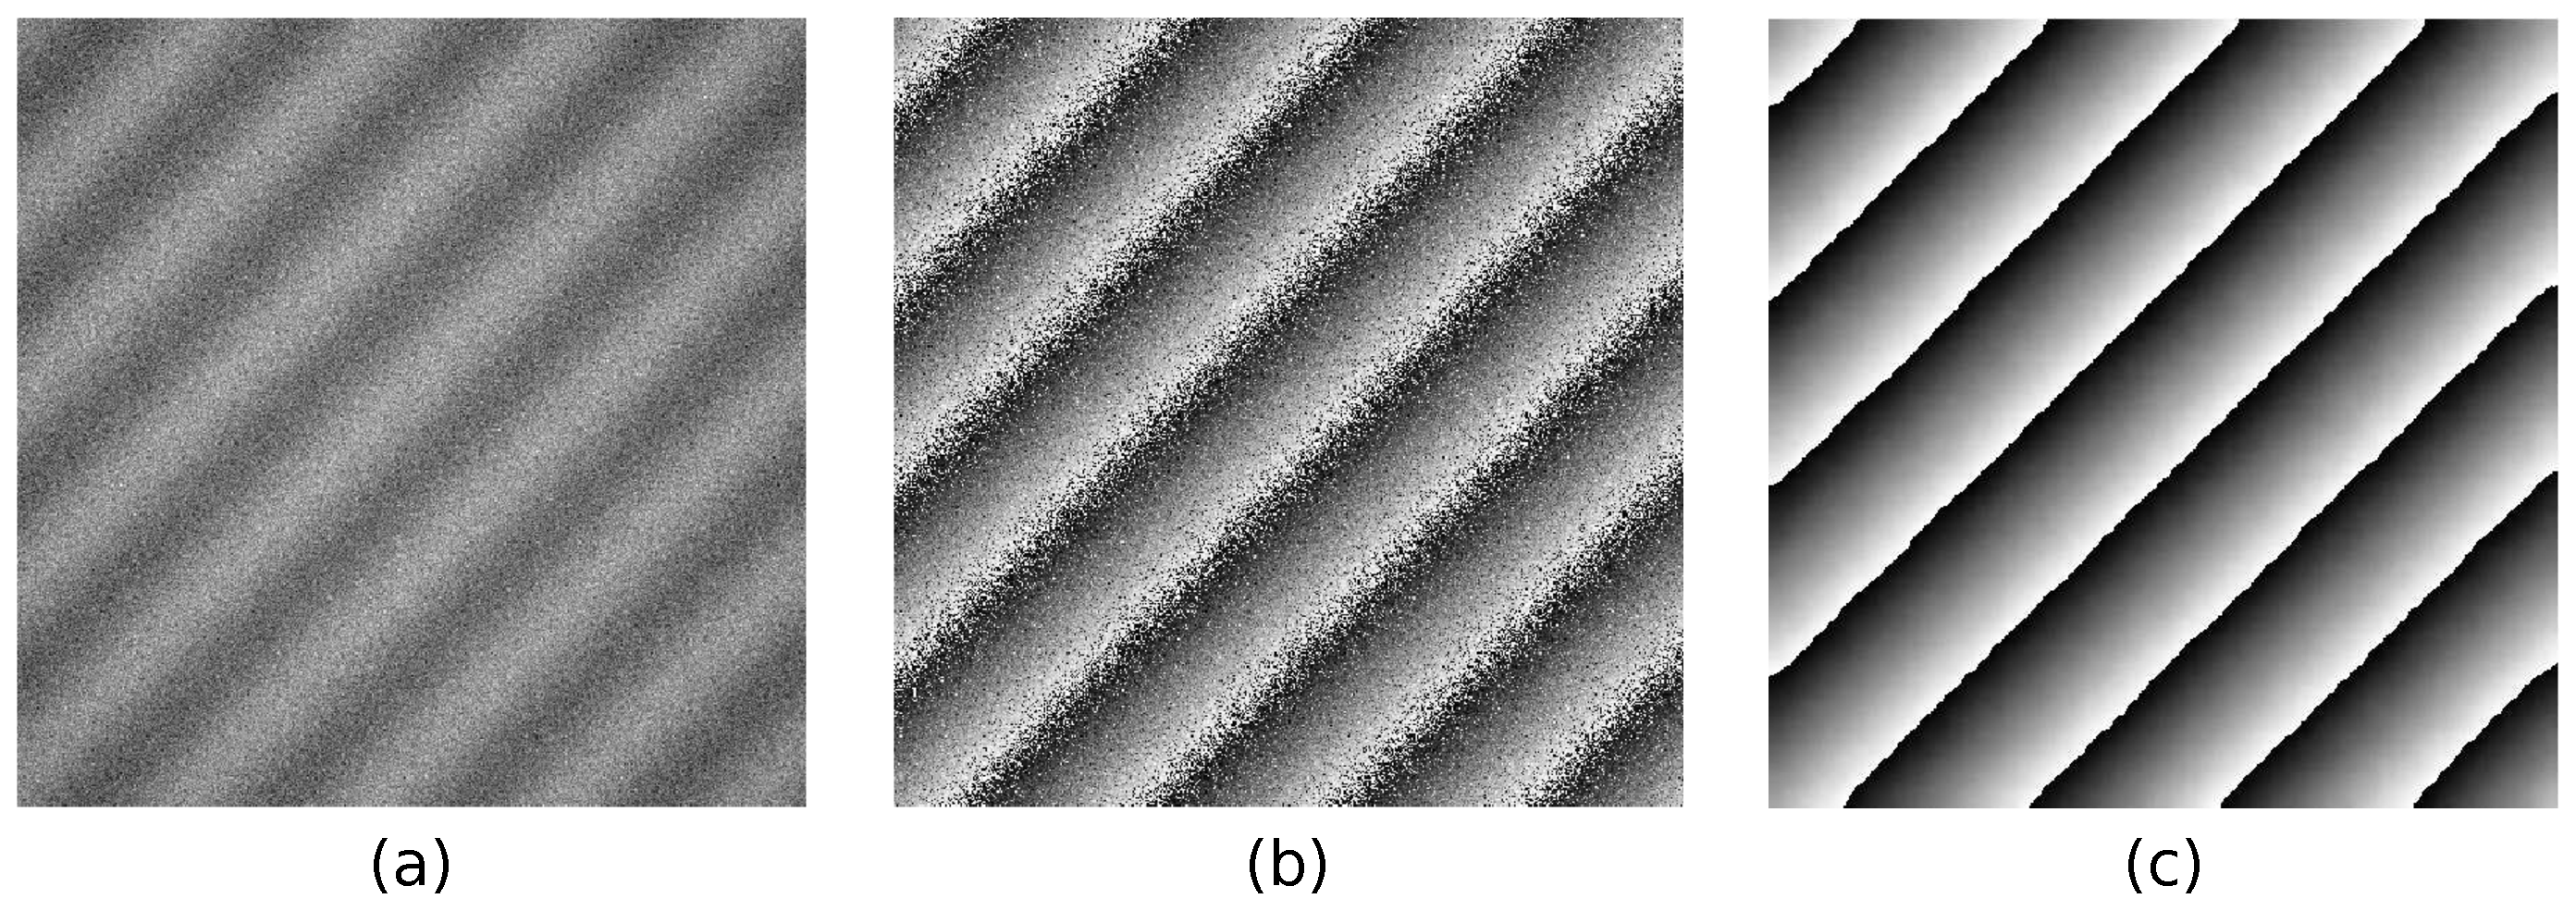
\includegraphics[scale=0.25]{Chpt1_figures/Fig_1.eps}
	\end{center}
	\caption{Numerical results. a) One of four experimental 
	interferogram sequences. b) Recovered phase map using classic 
	least-squares. c) Recovered phase map using our proposed 
	\textit{Full-field 2D least-squares}.}
	\label{fig:SimPhaseComparison}
\end{figure}
%%%%%%%%%%%%
\section{Numerical Experiments}
%%%%%%%%%%%%


To show the performance of the \textit{Full-field 2D least-squares} algorithm,
we simulated a PSI sequence of four interferograms of $512 \times 512$ pixels 
in the following way: $I(x,y,k) = a(x,y) + b(x,y) cos[\phi(x,y)+\alpha k] +
\eta(x,y)$, for $k=0,1,2,3$ and $\alpha=\pi/2$. The modulated phase $\phi$ was
modeled as a plane using the following expression: $\phi(x,y)=0.05x+0.05y$. The
background illumination term $a$ was modeled as a parabola centered at pixel
(256,256) of the image frames with a dynamic range between 0 and 1. The $b$ term
was set to $1$. Last, we added a random field of white noise $\eta$, with mean
$\gamma=0$ and variance $\sigma^2=1$. In Fig. \ref{fig:SimPhaseComparison}(a),
we see the first interferogram of the simulated sequence. Figures 
\ref{fig:SimPhaseComparison}(b) and \ref{fig:SimPhaseComparison}(c) show the
wrapped phase using classical least-squares and the
\textit{Full-field 2D least-squares} method, respectively. To estimate the
wrapped phase in Fig. \ref{fig:SimPhaseComparison}(c), we solve the linear
system in Eq. \eqref{eq:psi regularized} using the Gauss-Seidel method and
setting $\lambda$ and $\mu$ to 50. The number of iterations was 500. For
this example, the mask $M_{x,x}$ in Eq. \eqref{eq:psi regularized} is one over
all the image; since all the image it is valid information. Computational
time was 4.6934 seconds, on a PC with an Intel Core i7 processor and 8 GB RAM
memory . We can see in these figures that our proposed method recovers a phase
with much less noise than the classic least-squares method, given the
regularization terms in Eq. \eqref{eq:psi regularized}.
\begin{figure}[th!]
	\begin{center}
		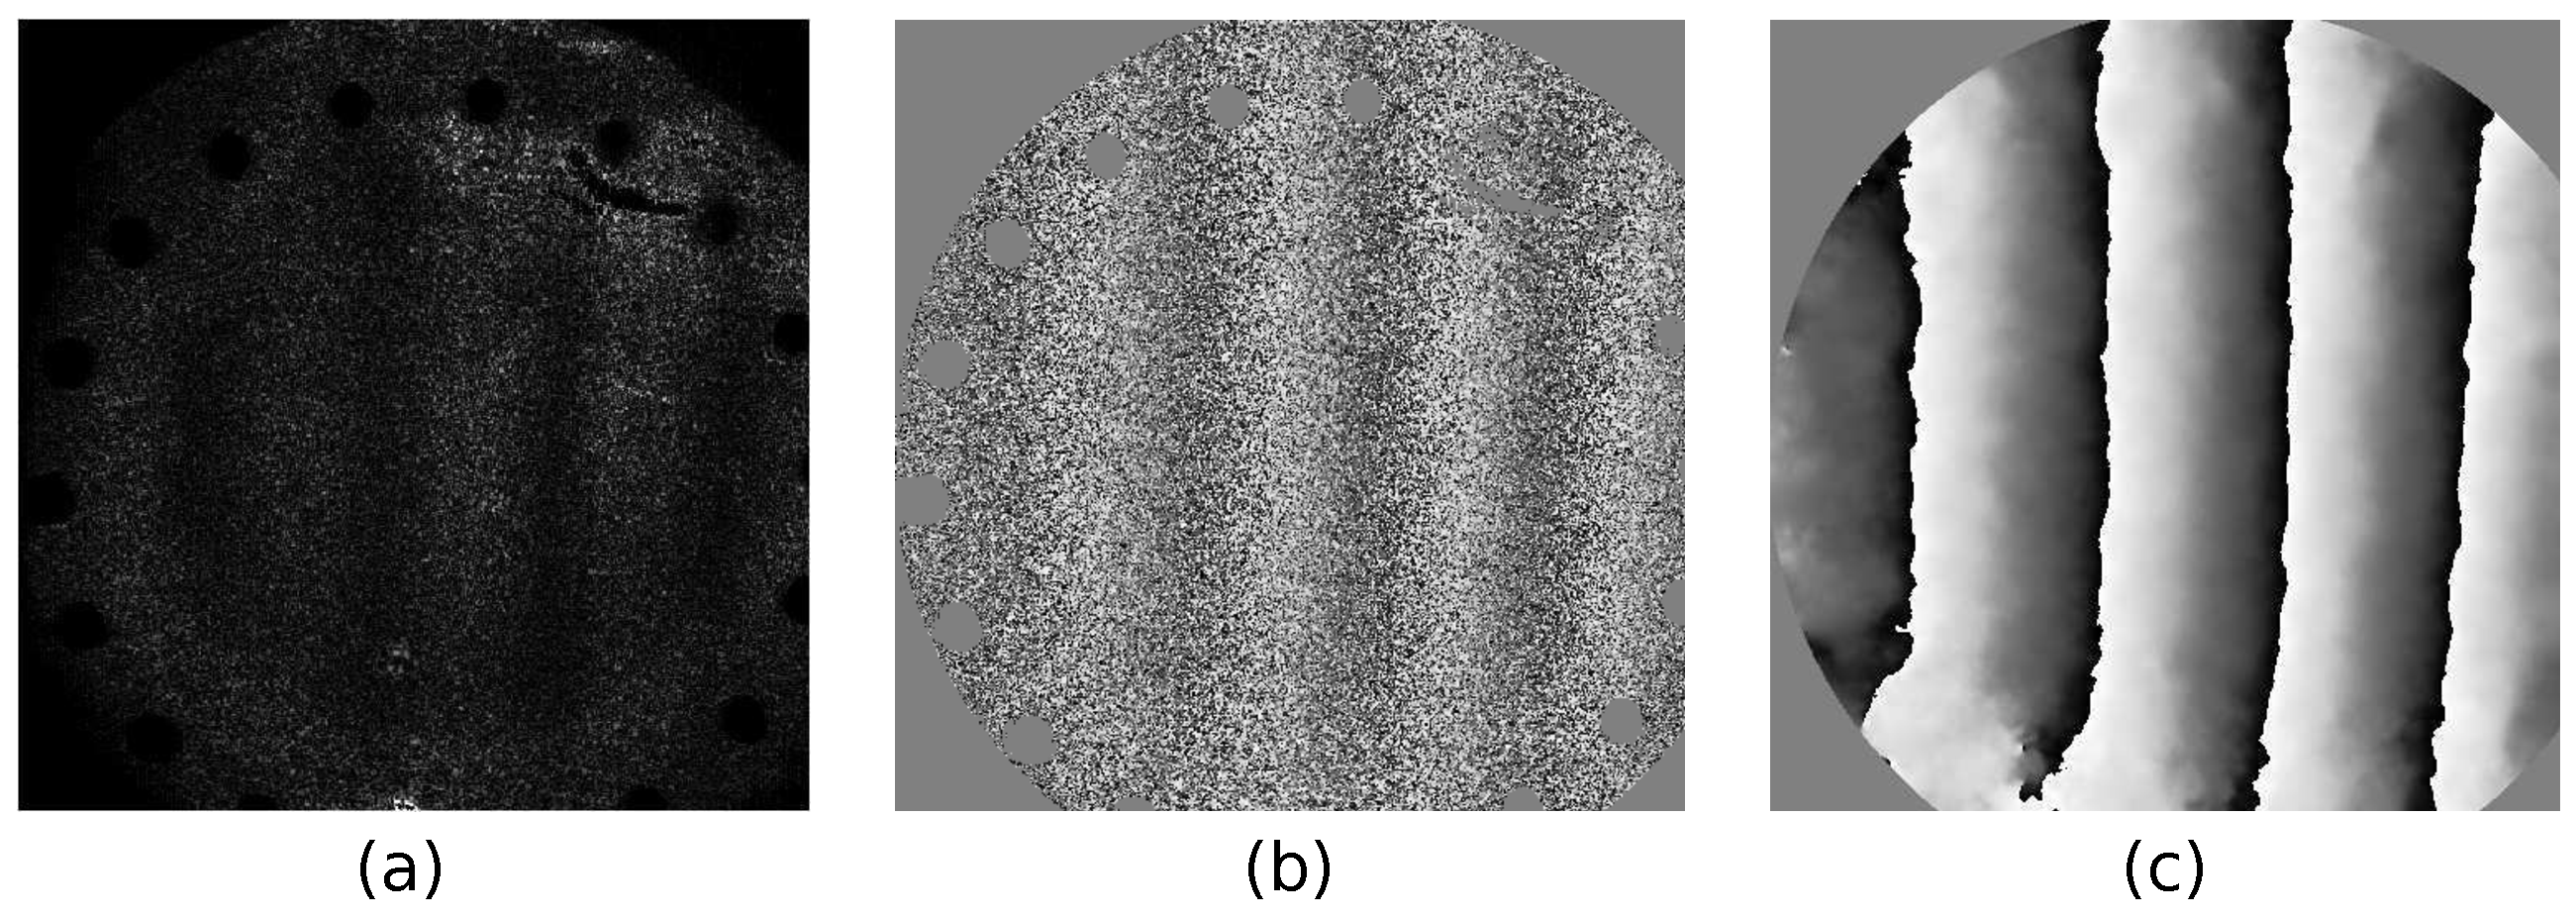
\includegraphics[scale=0.3]{Chpt1_figures/Fig_2.eps}
	\end{center}
	\caption{Experimental results. a) One of four experimental 
	interferogram sequences. b) Recovered phase map using classic 
	least-squares. c) Recovered phase map using our proposed 
	\textit{Full-field 2D least-squares}.}
	\label{fig:ExpPhaseComparison}
\end{figure}
%%%%%%%%%%%%
\section{Experimental Results}
%%%%%%%%%%%%

Now, we are going to show the performance of our method with experimentally 
obtained interferograms and compare it qualitatively with the classical 
least-squares method. The interferogram sequence was generated using an ESPI 
technique, and the wave-front under test was modified applying pressure. For 
the phase step, a phase-shift of $\pi/2$ radians was introduced. The object
under test was a circular metal plate with circular perforations all along
its edge. In order to increase reflexion, we coated the plate with white
powder, except for a small part, as can be seen in Fig.
\ref{fig:ExpPhaseComparison}(a). Fig. \ref{fig:ExpPhaseComparison}(a) shows the
first experimental phase-shifting interferogram of a 4 samples sequence. In
Fig. \ref{fig:ExpPhaseComparison}(b), we show the wavefront estimation of the 
classical least-squares method, while in Fig. \ref{fig:ExpPhaseComparison}(c), we 
see the wrapped phase estimation of the \textit{Full-field 2D least-squares} 
method proposed here. Computational time in this case was 7.6483 seconds
using the PC described above. As we can see, the proposed method was able to
estimate a phase free of noise. Another significant feature of this algorithm is
that in sections where there is no information, such as black circles and
scratches, the algorithm was able to fill-up the empty spaces satisfactorily;
this is because it takes into account the neighboring pixel information and the
regularization terms; very useful feature in the aforementioned cases.

%%%%%%%%%%%%
\section{Comments and conclusions}
%%%%%%%%%%%%

The calculation of a free-noise phase in PSI is very useful, since it allows 
us to use simple algorithms to unwrap the phase. Normally, to get a soft phase, 
we need to filter the interferogram samples or the output phase to 
remove the noise. The problem of this process is that we may be removing 
important information during the filtering. For this reason, the 
\textit{Full-field 2D least-squares} algorithm represents a significant 
improvement to the classical least-squares method. Besides, as we have seen
before, the presented algorithm is capable of interpolating small empty spaces
of missing data, since it takes into account the temporal and spatial
information. Therefore, all results presented in this paper can be directly
applied to the spatial case where missing data and discontinuities are present.
Examples of this are occlusions or shadows in projected fringe profilometry,
temporal decorrelation and saturated signal in heterodyne temporal
speckle-pattern interferometry.

Previous to this work, all phase-shifting algorithms only use a single pixel
signal to estimate the wave-front under test, regardless of adjacent
information. This chapter presents the usefulness of taking into account the
temporal and spatial information in conjunction to estimate a best phase
map. It is important to highlight that the functional of Eq. \eqref{eq:psi
regularized} is a linear system; therefore, it is stable and easy to compute. 
In conclusion, we present a full-field 2D linear demodulation algorithm  able 
to recover a clean phase and also able to interpolate small empty sections of
information, all with low computational time and in the same process.


%%%%%%%%%%%%%%%%%%%%%%%%%%%
%\begin{thebibliography}{99}
%%%%%%%%%%%%%%%%%%%%%%%%%%%
%\bibliographystyle{plain}
%\bibliography{./References_PhdThesis}


%% ---------------------------- classic PSI references 
  %\bibitem{Malacara} D. Malacara, M. Servin, and Z. Malacara, 
  %\textit{Interferogram Analysis for Optical Testing} (Taylor \& Francis, CRC, 
  %2005).
  
  %\bibitem{GeneralTheory} M. Servin, J. C. Estrada, and J. A. Quiroga, "The 
  %general theory of phase shifting algorithms," Opt. Express \textbf{17}(24), 
  %21867–21881 (2009) doi: http://dx.doi.org/10.1364/OE.17.021867.
  
  

 %%---------------------- Temporal PSI algorithms
  %\bibitem{RQF} J. Marroquin, J. Figueroa, and M. Servin, "Robust quadrature
  %filters," J. Opt. Soc. Am. A  \textbf{14}, 779-791 (1997).
  
  %\bibitem{temporal_1} P. D. Ruiz, J. M. Huntley, and G. H. Kaufmann, "Adaptive
  %phase-shifting algorithm for temporal phase evaluation," J. Opt. Soc. Am. A 
  %\textbf{20}(2), 325–332 (2003).
  
  %\bibitem{temporal_2}
  %P. Haible, M. P. Kothiyal, and H. J. Tiziani, “Heterodyne temporal 
  %speckle-pattern interferometry,” Appl. Opt. \textbf{39}(1), 114–117 (2000).
 
 

 
 %% ---------------- Regularized PSI and tuned algorithms
  
  %\bibitem{Mariano2} M. Rivera, R. Bizuet, A. Martinez, and J. Rayas,
  %"Half-quadratic cost function for computing arbitrary phase shifts and phase:
  %Adaptive out of step phase shifting," Opt. Express  1\textbf{4}, 3204-3213
  %(2006). http://dx.doi.org/10.1364/OE.14.003204
  
   
  
  %\bibitem{Medina} Orlando Medina, Julio C. Estrada and Manuel Servin 
  %"Regularized self-tuning phase demodulation for phase-shifting 
  %interferometry with arbitrary phase shifts", Proc. SPIE \textbf{8493},
  %Interferometry XVI: Techniques and Analysis, 84930K (September 13, 2012); 
  %doi:10.1117/12.929756.
  
  %\bibitem{Zeng} F. Zeng, Q. Tan, H. Gu, and G. Jin, "Phase extraction from 
  %interferograms with unknown tilt phase shifts based on a regularized optical
  %flow method," Opt. Express \textbf{21}, 17234-17248 (2013).
 

%% ------------------- Least-Squares references ---------------------
  %\bibitem{Morgan} C. Morgan, "Least-squares estimation in phase-measurement 
  %interferometry," Opt.  Lett. \textbf{7}, 368-370 (1982).
  
  %\bibitem{Greivenkamp} J. E. Greivenkamp "Generalized Data Reduction For 
  %Heterodyne Interferometry", Opt. Eng. \textbf{23(4)}, 234350 (Aug 01,
%1984).; 
  %http://dx.doi.org/10.1117/12.7973298

  %\bibitem{Okada} K. Okada, A. Sato, and J. Tsujiuchi, "Simultaneous 
  %calculation of phase distribution and scanning phase shift in phase 
  %shifting interferometry," Opt.  Commun. \textbf{84}, 118-124 (1991).
  
  %\bibitem{Kong} I.-B. Kong. "General algorithm of phase-shifting 
  %interferometry by iterative least-squares fitting". Opt. Eng., 
  %\textbf{34}:183, 1995.
 
%% ------------------- Marroquin references ---------------------

 
  %\bibitem{AQF} J. Marroquin, M. Servin, and R. Rodriguez-Vera,
  %"Adaptive quadrature filters and the recovery of phase from fringe
  %pattern images," J. Opt. Soc. Am. A \textbf{14}, 1742-1753 (1997).
  
  %\bibitem{AQF_mult} J. Marroquin, M. Servin, and R. Rodriguez Vera, 
  %"Adaptive quadrature filters for multiple phase-stepping images," Opt. 
  %Lett.  \textbf{23}, 238-240 (1998).

  %% ------------------- Regularized PSI references ---------------------
  %\bibitem{RPT} M. Servin, J. Marroquin, and F. Cuevas, "Fringe-follower 
  %regularized phase tracker for demodulation of closed-fringe interferograms," 
  %J. Opt. Soc. Am. A \textbf{18}, 689-695 (2001).
  
  %\bibitem{RQPT} M. Servin, J. Marroquin, and J. Quiroga, "Regularized
  %quadrature and phase tracking from a single closed-fringe interferogram," J. 
  %Opt. Soc. Am. A \textbf{21}, 411-419 (2004).
  
  %\bibitem{Mariano} R. Legarda-Saenz and M. Rivera, "Fast half-quadratic 
  %regularized phase tracking for nonnormalized fringe patterns," J. Opt. Soc. 
  %Am. A \textbf{23}, 2724-2731 (2006).
  
  %\bibitem{Vargas} J. Vargas, J. Quiroga, C. Sorzano, J. Estrada, and J.
%Carazo,
  %"Two-step interferometry by a regularized optical flow algorithm," Opt.
%Lett. 
  %\textbf{36}, 3485-3487 (2011).
  
  %\bibitem{Quiroga} J. Quiroga, J. Estrada, M. Servín, and J. Vargas, 
  %"Regularized least squares phase sampling interferometry," Opt. Express 
  %\textbf{19}, 5002-5013 (2011). http://dx.doi.org/10.1364/OE.19.005002
  
  %\bibitem{GPU} 
  %\linkable{http://en.wikipedia.org/wiki/Graphics\_processing\_unit}
  
%\end{thebibliography}

%\end{document}
